\documentclass[a4paper,12pt]{article} % тип документа

%  Русский язык
\usepackage[T2A]{fontenc}			% кодировка
\usepackage[utf8]{inputenc}			% кодировка исходного текста
\usepackage[english,russian]{babel}	% локализация и переносы

\usepackage{graphicx}               % импорт изображений
\usepackage{wrapfig}                % обтекаемые изображения
\graphicspath{{pictures/}}          % обращение к подкаталогу с изображениями
\usepackage[14pt]{extsizes}         % для того чтобы задать нестандартный 14-ый размер шрифта
\usepackage[warn]{mathtext}         % русский язык в формулах
\usepackage{indentfirst}            % indent first
\usepackage[margin = 25mm]{geometry}% отступы полей
\usepackage[table,xcdraw]{xcolor}   % таблицы
\usepackage{amsmath,amsfonts,amssymb,amsthm,mathtools} % Математика
\usepackage{wasysym}                % ???
\usepackage{upgreek}                % ???  
\usepackage{caption}
\captionsetup{labelsep=period}
\usepackage{mathrsfs}
\usepackage{makecell}
\usepackage{gensymb} % degree symbol



\pagestyle{empty}


\begin{document}
	\section*{Билет №11}
	\subsection*{Степенные ряды с комплексными числами}
	\noindent\textbf{Определение} $\sum\limits_{k = 0}^\infty c_k(\zeta - a)$; $c_k, a \in \mathbb{C} -$ фиксированные числа, $\zeta \in \mathbb{C}$  - переменная. \\
	Такой функциональные ряд называется \textit{степенным}.\\
	$c_k$ - коэф. степенного ряда. Этот ряд сходится в точке а.\\
	$\zeta - a = z \Rightarrow \sum\limits_{k = 0}^\infty c_k z^k$ - будем рассматривать такой степенной ряд, который сходится в т. $z = 0$ \\
	\subsection*{Теорема 1. [Первая теорема Абеля]}
	\noindent1. Если степенной ряд $\sum\limits_{k = 0}^\infty c_k z^k$ сходится в т. $z \neq 0$, то он сходится в круге: $k_0 = \{z = \mathbb{C}: |z| < |z_0|\}$ \\
	\noindent 2. Если степенной ряд $\sum\limits_{k = 0}^\infty c_k z^k$ расходится в т. $z_1$, то он расходится в любой т. $z: |z| > |z_1|$ \\
	\begin{figure*}[h!]
		\centering
	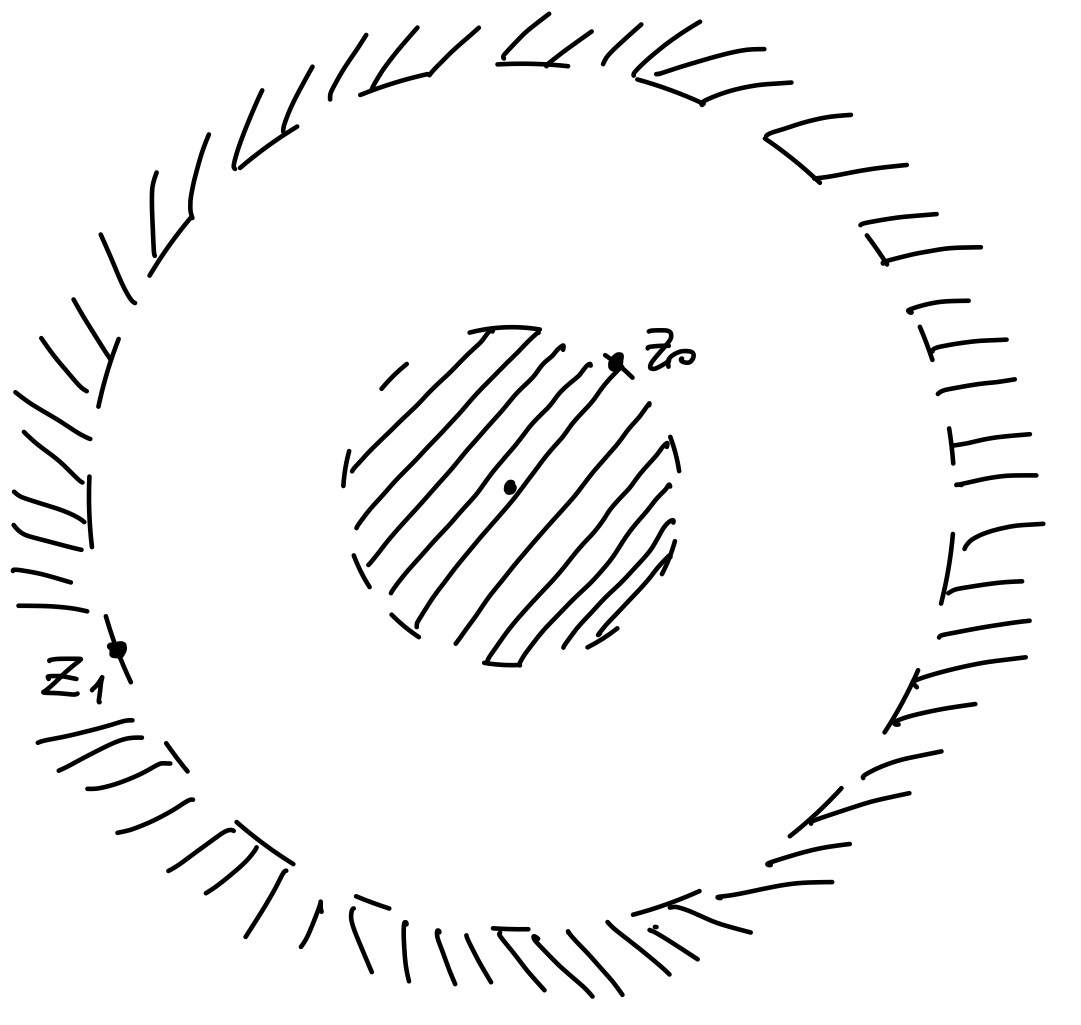
\includegraphics[scale = 0.1]{Que_11_pic_1.jpeg}
	\end{figure*}
\ \\
\noindent[$\lim\limits_{n \rightarrow \infty} z_n = a$] $ \stackrel{\text{def}}{=}$ [$\lim\limits_{n \rightarrow \infty} |z_n - a| = 0$] \\
\ \\
$\forall \varepsilon > 0 \quad\exists \, N = N (\varepsilon): \forall n \geqslant N \Rightarrow |z_n - a| < \varepsilon $ \\
\ \\
\noindent\textbf{Доказательство:} \\
\ \\
1) $\sum\limits_{k = 0}^\infty c_k z_0^k < \infty \Rightarrow c_k z_0^k \underset{k \to \infty}{\longrightarrow} 0 \Rightarrow \text{Ограничена:} \,  \exists M > 0: \forall k \Rightarrow |c_k z_0^k| \leqslant M$ \\
\ \\
$ \forall z: |z| < |z_0| $ \\
$ |c_k z^k| = | c_k z_0^k  \left(  \frac{z}{z_0} \right)^k | \leqslant M \cdot \left[ q(z) \right]^k, |q(z)| < 1 \Rightarrow \sum\limits_{k = 0}^\infty q^k(z) < \infty \Rightarrow
$\\
$
 \Rightarrow \sum\limits_{k = 0}^\infty |c_k z^k| < \infty \Rightarrow \sum\limits_{k = 0}^\infty c_k z^k
$\\
\ \\
2) $
\sum\limits_{k = 0}^\infty c_k z_1^k = \infty \Rightarrow \forall z: |z| > |z_1| - \text{ряд} \sum\limits_{k = 0}^\infty c_k z^k \text{ расходится, если бы в точке } z_2: 
$\\
$
|z_2| > |z_1| \text{ ряд } \sum\limits_{k = 0}^\infty c_k z_2^k < \infty \stackrel{1)}{\Rightarrow} \sum\limits_{k = 0}^\infty c_k z_1^k < \infty
$ - противоречие \\
\ \\
\noindent\textbf{Следствие 1. } Если $\sum\limits_{k = 0}^\infty c_k z_0^k < \infty, z_0 \neq 0$, то $\forall \rho: 0 < \rho < |z_0|$ в круге $k_{\rho} = \{z \in \mathbb{C} : |z| \leqslant \rho \} \text{ ряд } \sum\limits_{k = 0}^\infty c_k z^k$ сходится равномерно. \\
\ \\
\noindent\textbf{Доказательство:} \\
$
\exists M > 0: \forall k \Rightarrow |c_k z_0^k| \leqslant M
$ \\
\ \\
$ \forall z \in K_{\rho} $\\
\ \\
$
|c_k z^k| = |c_k z_0^k \cdot \frac{z^k}{z_0^k} | \leqslant M \left( \frac{\rho}{|z_0|} \right)^k = M \cdot q^k
$ \\
\ \\
$ |q| = \frac{\rho}{|z_0|} < 1 $ ($\frac{\rho}{|z_0|}$ не зависит от $z$), \\
\ \\
$\sum\limits_{k = 0}^\infty q^k < \infty \stackrel{\text{По пр. Вей.}}{\Rightarrow} \sum\limits_{k = 0}^\infty c_k z^k$ сходится равномерно в круге  $K_{\rho}$ \\
\ \\
\noindent\textbf{Следствие 2} Если в т. $z_0 \neq 0 $ вып. $\sum\limits_{k = 0}^\infty c_k z_0^k < \infty $, то \\
1) $\sum\limits_{k = m}^\infty c_k z^{k - m}$ сходится абсолютно в круге $K_0$ и равномерно в круге $K_{\rho}$ \\
2) $\sum\limits_{k = 1}^\infty k c_k z^{k - 1}$ сходится абсолютно в круге $K_0$ и равномерно в круге $K_{\rho}$ \\
\ \\
\noindent\textbf{Доказательство:} \\
1) $\forall z \in k_0 \Rightarrow |c_k z^{k - m} | = |c_k z_0^k \left(\frac{z}{z_0} \right)^{k - m} \cdot \frac{1}{z_0^m} | \leqslant$ \\
\ \\
$
 \frac{M}{|z_0|^m} \cdot | \frac{z}{z_0} |^{k-m} = \frac{M}{|z_0|^m} \cdot q^{k - m} (z), \quad q(z) = |\frac{z}{z0}| < 1
$\\
\ \\
$\sum\limits_{k = m}^\infty q^{k - m} < \infty $ - сходится абсолютно в $K_0$\\
\ \\
$ \forall z \in K_1 \Rightarrow |c_k z^{k - m}| \leqslant \frac{M}{|z_0|^m} \cdot q_1^{k - m}, \quad q_1 = \frac{\rho}{|z_0|} < 1.
$\\
\ \\
$0 < q_1 < 1$ - не зависит от $z$ $\Rightarrow$ по признаку Вейр. в $K_1$ ряд сходится равномерно\\
\newpage
\noindent2) $\forall z \in K_0$ \\
\ \\
$ |k c_k z^{k-1} | = | \frac{c_k z_0^k}{z_0} \cdot k\left( \frac{z}{z_0} \right)^{k-1} | \leqslant \frac{M}{|z_0|} \cdot  k q^{k - 1}(z), q(z) = | \frac{z}{z_0} | < 1 $ \\
\ \\
$ \sum\limits_{k = 1}^\infty k q^k(z) < \infty $ по признаку Даламбера\\
\ \\
\subsection*{Теорема 2. [О радиусе сходимости степенного ряда]}
\noindentДля любого степенного ряда существует $R \, \, (R \geqslant 0 \text{ или } R = +\infty)$\\
 такое, что \\
 1) $0 < R < \infty \Rightarrow \sum\limits_{k = 0}^\infty c_k z^k < \infty$ в круге $K = \{ z \in \mathbb{C} : |z| < R\}$ и расходится в $\mathbb{C} \backslash \overline{K}$\\
 2)$R = 0$, то $\sum\limits_{k = 0}^\infty c_k z^k < \infty$ только в $z = 0$\\
 3) $R = +\infty$, то $\sum\limits_{k = 0}^\infty c_k z^k < \infty \  \forall z \in \mathbb{C}$\\
 $R$ - называется радиусом сходимости степенного ряда $\sum\limits_{k = 0}^\infty c_k z^k$ \\
 $K$ - круг сходимости\\
 \ \\
 \noindent\textbf{Доказательство:} Пусть $\mathscr{D} \subset \mathbb{C}$ - множество сходимости степенного ряда; $\mathscr{D} \neq \varnothing$, т.к. $0 \in \mathscr{D}$\\
 \ \\
 1) $\mathscr{D}$ - огран., $z_0 \in \mathscr{D}, z_0 \neq 0$ \\
 \ \\
 $R = \underset{z \, \in \, \mathscr{D}}{\sup} |z| $ - сущ. т.к. $\mathscr{D}$ огранич. мн-во.\\
 \ \\
 Докажем: $\forall \  z \in K \Rightarrow  \sum\limits_{k = 0}^\infty c_k z^k < \infty$ \\
 \ \\
 $\forall z \in \mathbb{C} \backslash \overline{K} \Rightarrow  \sum\limits_{k = 0}^\infty c_k z^k = \infty$\\
 \ \\
 По определению $\sup \, \forall z'\in K \  \exists z_1 \in \mathscr{D} : |z'| < |z_1| \leqslant R$, т.к. \\
 \ \\
 $ \sum\limits_{k = 0}^\infty c_k z_1^k < \infty \Rightarrow$ 1-я теорема Абеля $ \sum\limits_{k = 0}^\infty c_k (z')^k < \infty$ и сходится абсолютно $\Rightarrow$ В силу произв. $z' \in K \Rightarrow  \sum\limits_{k = 0}^\infty c_k z^k$ сходится абс. в круге $K$\\
 \ \\
 Пусть $z' \notin K \Rightarrow |z'| > R \Rightarrow$ по опред. $\sup z' \notin \mathscr{D} \Rightarrow  \sum\limits_{k = 0}^\infty c_k (z')^k = \infty \Rightarrow$ расходится вне круга $K$\\
 \ \\
 2) $\mathscr{D}$ - огран.;  если $\mathscr{D} = \{0\}$, то ряд сход в т. $z = 0$ и расх в $z \neq 0$\\
 \ \\
 $ \sum\limits_{k = 0}^\infty c_k z^k < \infty \quad z = 0 \quad \Rightarrow R = 0$\\
 \ \\
 3) $\mathscr{D}$ - неогранич. $\Rightarrow \forall z \in \mathbb{C} \  \exists z'  \in \mathscr{D}:$\\
 \ \\
 $|z| < |z'|,  \sum\limits_{k = 0}^\infty c_k (z')^k < \infty \stackrel{\text{1-я т. Аб.}}{\Rightarrow}  \sum\limits_{k = 0}^\infty c_k z^k < \infty$\\
 \subsection*{Теорема 3. [Вторая теорема Абеля]}
 \noindent Если $0<R<+\infty, \  R$ - радиус сходимости $\sum\limits_{k = 0}^\infty c_k z^k$  и $\sum\limits_{k = 0}^\infty c_k R^k < \infty$, то на $[0, R]$ ряд $\sum\limits_{k = 0}^\infty c_k z^k$ сх. равномерно и его сумма $S(x) = \sum\limits_{k = 0}^\infty c_k x^k$ непрерывна $\forall x \in [0, R]$\\
 \ \\
\noindent\textbf{Доказательство:}\\
$ \sum\limits_{k = 0}^\infty \underbrace{c_k R^k}_{U_k} \cdot \underbrace{\left(\frac{x}{R}\right)^k}_{V_k} =
$ \\
1) $\sum\limits_{k = 0}^\infty c_k R^k < \infty $ \\
\ \\
2) $V_k =  \left( \frac{x}{R} \right)^k \quad 0 \leqslant V_k \leqslant 1 \quad \forall x \in [0; R]$ \\
\ \\
  $V_{k + 1} = \left( \frac{x}{R} \right)^{k + 1}  < \left( \frac{x}{R} \right)^k = V_k \quad \forall k$\\
\hspace*{3 cm}$\Downarrow$ признак Абеля \\
$\sum\limits_{k = 0}^\infty c_k x^k < \infty$ сходится равномерно на $[0, R]$\\
$f_k(x) = c_k x^k$  - непрерывна на $[0; R]$\\
\hspace*{3 cm}$
\Downarrow
$\\
$
S(x) = \sum\limits_{k = 0}^\infty c_k x^k$ непреревна на $[0; R]$\\
 \subsection*{Теорема 4.}
 $\sum\limits_{k = 0}^\infty c_k z^k$ \\
 1) $\lim\limits_{k \to \infty} \sqrt[k]{|c_k|} = \rho \quad (\rho \geqslant 0,\, \rho = +\infty) \Rightarrow R =  \frac{1}{\rho}$ \\
 \ \\
 2) Если $|c_k| > 0 \  \forall k \text{ и } \lim\limits_{k \to \infty} \frac{|c_{k+1}|}{|c_k|} = \rho \ (\rho \geqslant 0, \rho = +\infty) \Rightarrow R = \frac{1}{\rho}$\\
 \ \\
 \noindent\textbf{Доказательство:}\\
 \ \\
 $K = \{z \in \mathbb{C}: |z| < \frac{1}{\rho} \}$ \\
 \ \\
 $z_0 \in K: \sqrt[k]{|c_k z_0^k|} = |z_0| \sqrt[k]{|c_k|} \underset{k \to \infty}{\longrightarrow} |z_0| \cdot \rho < \frac{1}{\rho} \cdot \rho = 1 $\\
\hspace*{3 cm} $\Downarrow$ По признаку Коши \\
\hspace*{3 cm}$\sum\limits_{k = 0}^\infty |c_k z_0^k| < \infty$\\
\ \\
$z_1: |z_1| > \frac{1}{\rho}$\\
\ \\
$\sqrt[k]{|c_k z_1^k|} = |z_1| \sqrt[k]{|c_k|} \underset{k \to \infty}{\longrightarrow} |z_1| \cdot > \frac{1}{\rho} \cdot \rho \Rightarrow
$ По признаку Коши $\sum\limits_{k = 0}^\infty c_k z_1^k = \infty$\\
\ \\
\noindent\textbf{Пример (показывает, для чего нужна формула Коши-Адамара):}\\
$\sum\limits_{k = 1}^\infty z^{k^2} = z + z^4 + z^9 + z^{16} + z^{25} + .... + z^{k^2} + ...
$\\
\ \\
$ \{c_k\} = \{ c_1 = 1, c_2 = c_3 = 0, c_4 = 1, c_5 = c_6 = c_7 = c_8 = 0, c_9 = 1, ... \} $\\
\ \\
$\overline{\lim\limits_{k \to \infty}} \sqrt[k]{|c_k|} = \lim\limits_{k \to \infty} \sqrt[k^2]{|c_{k^2}|} = 1 \Rightarrow R = 1 $
\subsection*{Теорема 5. [Формула Коши-Адамара]}
\noindent Если $R$ - радиус сходимости $\sum\limits_{k = 0}^\infty c_k z^k$, тогда \\
$ R = \frac{1}{\overline{\lim\limits_{k \to \infty}} \sqrt[k]{|c_k|}} $\\
\ \\
\noindent\textbf{Доказательство:}\\
1) $ \{ \sqrt[k]{|c_k|}\} $ - неогр. \\
\ \\
2) $ \overline{\lim\limits_{k \to \infty} }\sqrt[k]{|c_k|}  = L > 0; \quad L \in R$\\
\ \\
3) $ \overline{\lim\limits_{k \to \infty} }\sqrt[k]{|c_k|}  = 0 \Rightarrow \{ \sqrt[k]{|c_k|}\}$ сходится к 0\\
\ \\
1) Для бескон. числа номеров $k \in \mathbb{N}$ \\
\indent$|c_k z^k| > 1 \quad \forall z \neq 0, \  z \in \mathbb{C}$ \\
\hspace*{3 cm} $\Downarrow$\\
Не выполняется необходимое условие сходимости ряда \\
\hspace*{3 cm} $\Downarrow$\\
\hspace*{2 cm} $\sum\limits_{k = 0}^\infty c_k z^k = \infty $\\
\hspace*{3 cm} $\Downarrow$\\
\hspace*{1.9 cm} $\sum\limits_{k = 0}^\infty c_k z^k < \infty \ $ только для $z = 0$\\
\ \\
2) Докажем, что\\
а) $\forall z: |z| < \frac{1}{L}$ ряд сходится \\
б) $\forall z: |z| < \frac{1}{L}$ ряд расходится\\
\ \\
а) $z: \quad |z| < \frac{1}{L}$ \\
Тогда $\exists \, \varepsilon > 0: |z| < \frac{1}{L + \varepsilon} < \frac{1}{L} $\\
\ \\
$\varepsilon > 0 \  \exists \, k_0(\varepsilon): \forall k \geqslant k_0 \Rightarrow \sqrt[k]{|c_k|} < L + \frac{\varepsilon}{2}
$ \\
\ \\
$ \sqrt[k]{|c_k z^k|} = |z| \sqrt[k]{|c_k|} \leqslant \frac{L + \frac{\varepsilon}{2}}{L + \varepsilon}
$\\
\hspace*{1 cm} $\Downarrow$ По признаку Коши\\
$\sum\limits_{k = 0}^\infty c_k z^k < \infty \ $ в круге $K = \{z: |z| < \frac{1}{L}\}$\\
\ \\
б) $\forall z: |z| > \frac{1}{L} \Rightarrow \exists \, \varepsilon > 0: |z| > \frac{1}{L - \varepsilon} > \frac{1}{L} $\\
$[\   \exists \  \{c_{k_n}\} : \lim\limits_{n \to \infty} \sqrt[k]{|c_k|} = L \,] \stackrel{\text{def}}{=} [\varepsilon > 0 \  \exists \, n_0 : \forall n \geqslant n_0 \Rightarrow L - \varepsilon < \sqrt[k_n]{|c_{k_n}|} \,]$ \\
\ \\
$\sqrt[k_n]{|c_{k_n}| z^{k_n}} = |z| \sqrt[k_n]{|c_{k_n}|} > \frac{1}{L - \varepsilon} \cdot (L - \varepsilon) = 1 \quad \forall n \geqslant n_0  \Rightarrow |c_k z^{k_n}| > 1 \Rightarrow$\\ 
\ \\
$\Rightarrow$ Не выполняется необходимых условий сходимости \\
\hspace*{3 cm} $\Downarrow$\\
 Ряд расходится $\forall z: |z| > \frac{1}{L}$\\
 \ \\
 3) $\overline{\lim\limits_{k \to \infty} }\sqrt[k]{|c_k|} = 0 \Rightarrow \{ \sqrt[k]{|c_k|}\}$ сходится к 0.\\
 \ \\
 $\forall z \in \mathbb{C}, \   z \neq 0 : \frac{1}{2|z|} = \varepsilon: \quad  \exists \, k_0(\varepsilon) : \forall k \geqslant k_0 \Rightarrow \sqrt[k]{|c_k|} < \frac{1}{2|z|} \Rightarrow$\\
 \ \\
 $\Rightarrow \sqrt[k]{|c_k|\cdot |z^k|} = |z|\sqrt[k]{|c_k|} < |z| \cdot \frac{1}{2|z|} = \frac{1}{2} < 1$ \\
 \hspace*{1 cm} $\Downarrow$ По признаку Коши\\
 $\sum\limits_{k = 0}^\infty c_k z^k  < \infty \quad \forall z \in \mathbb{C}$
 \subsection*{Свойства степенных рядов}
  \subsection*{Теорема 7.}
  \noindent Для рядов \\
  \ \\
  $\sum\limits_{k = 0}^\infty c_k z^k, \quad \quad \sum\limits_{k = 0}^\infty \frac{c_k z^{k + 1}}{k + 1}, \quad \quad \sum\limits_{k = 0}^\infty k c_k z^{k - 1} \quad$ \\
   \hspace*{0.5 cm}1) \hspace*{2.4 cm}2)\hspace*{2.7 cm}3)\\
   \ \\
    радиус сходимости один и тот же.\\
    1) $R_1, K_1$\\
    2) $R_2, K_2$\\
    3) $R_3, K_3$\\
    Надо доказать: $R_1 = R_2 = R_3 = R$\\
\ \\
    \noindent\textbf{Доказательство:}\\
    $\forall k \in \mathbb{N} \Rightarrow \frac{1}{k + 1} < 1 \leqslant k \quad  \times |c_k z^{k + 1}|$\\
    \ \\
    $|\frac{c_k}{k + 1} z^{k + 1}| \leqslant |z| \cdot |c_k z^k| \leqslant |z|^2 \cdot |k c_k z^{k - 1}|$\\
    \ \\
    $\underbrace{ |z| \cdot |c_k z^k| \leqslant |z|^2 \cdot |k c_k z^{k - 1}|}_{1)} \quad \quad \underbrace{|\frac{c_k}{k + 1} z^{k + 1}| \leqslant |z| \cdot |c_k z^k|}_{2)}$\\
    1) $\forall z \neq 0 \in K_3 \Rightarrow \sum\limits_{k = 0}^\infty c_k z^k < \infty \Rightarrow R_1 \geqslant R_3$\\
    2) $\forall z \neq 0 \in K_1 \Rightarrow \sum\limits_{k = 0}^\infty \frac{c_k}{k + 1} z^{k+1} < \infty \Rightarrow R_1 \leqslant R_2$\\
    \ \\
    В результате: $R_3 \leqslant R_1 \leqslant R_2 $\\
    \ \\
    Надо доказать, что $R_2 \leqslant R_3$\\
    \ \\
    $z \in K_2 \ \  \exists \, \rho < R_2: z \in K_{\rho} \quad |k c_k z^{k - 1}| = |k c_k z^{k - 1} \cdot \frac{k + 1}{k + 1} \cdot \frac{z^2}{z^2}|$ = \\
    \ \\
    $|\frac{c_k}{k + 1} \cdot z^{k + 1} \cdot \frac{k(k+1)}{z^2}| = | \frac{c_k}{k + 1} \cdot \rho^{k + 1} \cdot \frac{k(k + 1)}{z^2} \cdot \left( \frac{z}{\rho} \right)^{k + 1}| \stackrel{\exists M > 0}{\leqslant} $\\
    \ \\
    $\leqslant \frac{M}{|z|^2} k(k+1) \rho_1^{k + 1}, \text{ где } |q_1| < 1 \quad q_1 = \frac{z}{\rho}$    \\
    \hspace*{3 cm} $\Downarrow$\\
    $\forall \in K_2 \Rightarrow \sum\limits_{k = 0}^\infty k c_k z^{k - 1} < \infty \Rightarrow R_3 \geqslant R_2$\\
    Тогда в сумме $R_1 = R_2 = R_3 = R$\\
      \subsection*{Теорема 8.}
      \noindentЕсли $R$ - радиус степенного ряда $\sum\limits_{k = 0}^\infty a_k (x - a)^k = f(x), $\\
      $
      \quad x \in (a - R; a + R); \quad a_k, a, x \in R$, то\\
      \ \\
      1) $f$  бесконечно дифф. на $(a - R; a + R)$ \\
      $f^{(m)}(x) = \sum\limits_{k = m}^\infty k(k-1) ... (k - (m - 1)) a_k (x - 1)^{k - m}$ \\
      
      2) $\forall x \in (a - R; a + R) \Rightarrow \int_{a}^{x} f(t) dt = \sum\limits_{k = 0}^\infty \frac{a_k}{k + 1} (x - a)^{k + 1}$ \\
      \ \\
      При почленном дифференцировании ряда радиус не меняется.\\
      \ \\
      \textbf{Доказательство:}\\
      $\forall \rho: 0 < \rho < R  \text{ на } [a - \rho; a + \rho ]$ равномерная сходимость $\Rightarrow$ всё можно делать.\\
      \ \\
      \textbf{Следствие:}\\
      $a_k = \frac{f^{(k)(a)}}{k!}
	  $      
  
 
\end{document}